\begin{frame}
  {\Huge\insertsection{}}
  \begin{itemize}
    \item \cite{sabbah_cimpa90} §2.2.2 Asymptotic expansions
    \item \cite{van2003galois} Chap. 7 Exact Asymptotics
  \end{itemize}
  and
  \begin{itemize}
    \item \cite{majima1984asymptotic}
    \item \cite{zbMATH00060600}
    \item \cite{wasow2002asymptotic}
  \end{itemize}
\end{frame}

\begin{frame}
  Let \textcolor{red!60!black}{$U$} be an open interval in $S^1$
  \begin{itemize}
    \item $\Delta_r^*(U):=
      \{z\in\Delta_r\mid z=\rho e^{i\theta},0<\rho<r,\theta\in U\}$%
\footnote{$\Delta_r:=\Delta_r^*(S^1)$}
  \end{itemize}
  \begin{center}
    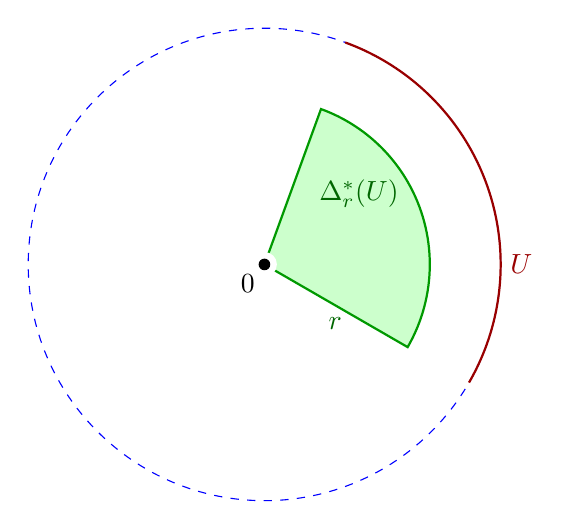
\begin{tikzpicture}[scale=3]
      \node (zero) at (0,0) {};
      \node[below left] at (zero) {$0$};
      \draw[blue,dashed] (zero) circle (1cm);

      \filldraw[fill=green!20!white,draw=green!60!black,thick] (0,0)
        -- ({cos( -30 )*.7},{sin( -30 )*.7}) arc (-30:70:.7) -- cycle;
      \node[green!40!black] at (.4,.3) {$\Delta_r^*(U)$};
      \node[green!40!black] at (.3,-.25) {$r$};

      \draw[thick,red!60!black] ({cos( -30 )},{sin( -30 )}) arc (-30:70:1);

      \node[red!60!black,right] at (1,0) {$U$};

      \fill[white] (zero) circle (1.5pt);
      \fill (zero) circle (.7pt);
    \end{tikzpicture}
  \end{center}
\end{frame}

\begin{frame}{Asymptotic expansion}
Let $\hat\phi=\sum_{n\geq-n_0}a_nx^n$ with $a_n\in\C$ is as asymptotic
expansion of $f$ at $0$ if for all $m\in\N$ one has
\begin{equation} \label{eq:asymptoticExpansion}
  \lim_{x\to 0,x\in\triangle_r^*(U)}
  \left|x^{-m}\right|\left|x^{n_{0}}f(x)-\sum_{0\leq n\leq m}a_{n}x^{n}\right|
  =0
\end{equation}
Define
\begin{itemize}
  \item $\bar\cA(U,r)\subset\cO(\Delta_r^*(U))$ the set of functions which
    admits an asymptotic power series
  \item $\cA(U,r):=\bigcap_{V}\bar\cA(V,r)$ where $V$ are relatively
    compact open subsets of $U$
    \begin{itemize}
      \item $\cA(U,r)=\{\phi\in \bar\cA(U,r)
        \mid \phi\in \bar\cA(V,r)
        \forall V\text{ rel.\  cp.\  op.\  subset of }U\}$
    \end{itemize}
  \item $\cA(U):=\bigcup_r\cA(U,r)$%
    \begin{itemize}
      \item $\cA(U)=\{\phi\mid\exists r\text{: } \phi\in\cA(U,r)\}
        =\{\phi\mid\exists r\text{: }
          \forall V\subset U\text{ rel.cp.op.}\text{: }
          \phi\in\bar\cA(V,r)\}$
    \end{itemize}
\end{itemize}
The mapping $U\mapsto\cA(U)$ defines a sheaf on $S^1$
\end{frame}

\begin{frame}
\begin{probl}
\begin{itemize}
  \item are there any restrictions to the coefficients $a_{-n_0},\dots,a_{-1}$?
\end{itemize}
\end{probl}
Take a look at $f=\frac{1}{x}$ and restrict to $\theta=0$ ($\R_{>0}$), then:
\[
  \forall m : \qquad
  \lim_{x\to 0,x\in\R_{>0}}
  \left|x^{-m}\right|\left|\frac{x^{n_{0}}}{x}
    -\sum_{0\leq n\leq m}a_{n}x^{n}\right| =0
\]
In the case $m=0$ we get $\left|\frac{x^{n_{0}}}{x} -a_{0}\right|\to0$. This
implies $n_0\geq1$, lets take $n_0=1$ and $a_0=1$.

In the case $m=1$ we get
$\frac{\left|\frac{x}{x} -1 -a_1x\right|}{|x|}\to0$

Thus
$ \left|\frac{x}{x^2} -\frac{1}{x} -a_1\right|\to0 $

Thus
$ \left|\frac{1}{x} -\frac{1}{x} -a_1\right|\to0$ Thus $a_1=0$ and so on
\end{frame}

{\setbeamercolor{background canvas}{bg=gray!40!white}
  \begin{frame}{Other definitions}
    \begin{itemize}
      \item \cite[2]{majima1984asymptotic} says:
        $f\in\cA(U)$ iff for every \textbf{closed} subsector and for every
        $N\in\N$
        \[
          \sup_{x\in\bar\cA(V,\tilde r)}
            \left|x^{-N}\left(f(x)-\sum_{i=0}^{N-1}a_ix^i\right)\right|
          <+\infty
        \]
      \item \cite{wasow2002asymptotic} defines:
        Let the function $f(x)$ be defined in a point-set $S$ of the complex
        $x$-plane having $x=0$ as an accumulation point. The power series
        $\sum_{r=0}^\infty a_rx^r$ is said to represent $f(x)$ asymptotically,
        as $x\to0$ is $S$, if
        \[
          x^{-m}\left[f(x)-\sum_{r=0}^ma_rx^r\right]
        \]
        tends to zero, for all $m\geq0$, as $x$ tends to zero in $S$.
      \item \cite{zbMATH00060600} defines:
        \textbf{asymptotic expansion of Grevrey order $s$}
        \begin{itemize}
          \item see: the following slides
        \end{itemize}
    \end{itemize}
  \end{frame}

  \begin{frame}{Definition from \cite{zbMATH00060600}}
  \begin{defn}
    $f=\sum_ma_mx^m$ is of Grevrey order $s$ (nonegative) :\Leftrightarrow
    \begin{itemize}
      \item there exist $C$ and $A$ nonegative such that
      \[
        |a_m|< C(m!)^sA^m \qquad \text{ for } m=0,1,2,\dots
      \]
    \end{itemize}
    We denote by $\C\llbracket z\rrbracket_s$ the set of all power series of
    Grevrey order $s$.
  \end{defn}
  \begin{defn}
  $\phi$ is said to admit an asymptotic expansion of Grevrey order $s$ as
  $z\to0$ on
  \[
    \mathcal{D}(R_0,a,b):=\{z \mid a < \arg z < b , 0 < |z| < R_0\}
  \]
  if
  \begin{itemize}
    \item $\phi$ is holomorphic on $\mathcal{D}(R_0,a,b)$
    \item there exists a formal power series
    $f=\sum_{m\geq0}a_mz^m \in \C\llbracket z\rrbracket_s$ such that
    \[
      \left|\phi(z)-\sum_{N-1\geq m\geq 0}a_mz^m\right|
      \leq K_{R,\alpha,\beta}(N!)^s(B_{R,\alpha,\beta})^N|z|^N
    \]
    on $\mathcal{D}(R,\alpha,\beta)$ for $N=1,2,\dots$ and every
    $(R,\alpha,\beta)$ satisfying
    \[
      0 < R < R_0 \qquad \text{ and } \qquad a < \alpha < \beta < b,
    \]
    where $K_{R,\alpha,\beta}$ and $B_{R,\alpha,\beta}$ are some nonegative
    numbers depending on $(R,\alpha,\beta)$.
  \end{itemize}
  \end{defn}
  \end{frame}

  \begin{frame}{Definition from \cite{zbMATH00060600} (2)}
    \begin{itemize}
      \item We denote by $\mathcal{A}_s(R_0,a,b)$ the set of all functions
      admitting asymptotic expansions of Grevrey $s$ as $z\to 0$ on the
      sectorial domain $\mathcal{D}(R_0,a,b)$.
      \item We set $J(\phi)=f$. Then the mapping
      \[
      J: \mathcal{A}_s(R_0,a,b) \to \C\llbracket z\rrbracket_s
      \]
      is a homomorphism of commutative differential algebras over $\C$.
      \item Set
      \[
      \mathcal{A}_{s,0}(R_0,a,b):=
      \ker\left(J: \mathcal{A}_s(R_0,a,b) \to \C\llbracket z\rrbracket_s\right)
      \]
    \end{itemize}
    \begin{lem}[1.3]
      A function $\phi(z)$ belongs to $\mathcal{A}_{s,0}(R_0,a,b)$ iff \dots
    \end{lem}
    \begin{cor}[1.4]
      $J$ is injective iff \dots
    \end{cor}
    \begin{defn}[1.5]
      Let $k$ be a positive number. A formal power series $f\in\C\llbracket
      z\rrbracket$ is \emph{k-summable in a direction} $\arg z=d$\dots 
    \end{defn}

    \dots

    \textbf{2. Grevrey properties of formal solutions:} We can define the
    Newton polygon\dots 
  \end{frame}
}

\begin{frame}{Some elementary properties (2.2.4)}
  \begin{enumerate}
    \item If $\hat\phi$ is an Asymptotic expansion for $f$ then one has
      \[
        a_0=\lim_{x\to 0,x\in\Delta_r^*(U)}x^{n_0}f(x)
      \]
      and for $m>0$,
      \[
        a_m=\lim_{x\to 0,x\in\Delta_r^*(U)}x^{-m}
          \left[x^{n_0}f(x)-\sum_{0\leq n\leq m-1}a_nx^n\right]
      \]
      In particular this asymptotic expansion is unique
      \begin{itemize}
        \item $f$ admits a zero asymptotic expansion iff for all $p\in\Z$
          one has
          \[
            \lim_{x\to 0,x\in\Delta_r^*(U)}x^pf(x)=0
          \]
      \end{itemize}
    \item
      Define $\cA(U)\to \hat K$ denoted by $f\mapsto \hat{f}$.
      \begin{itemize}
        \item $\cA(U)$ is a subring of $\cO(\Delta_r^*(U))$
        \item this mapping is a morphism of rings
      \end{itemize}
    \item Denote by $\cA^{<0}(U)$ the kernel of this morphism
      \begin{itemize}
        \item $x\mapsto e^{-\frac{1}{x}}$ has zero asymptotic expansion in
          some sector around $\theta=0$
      \end{itemize}
    \item $\cA(U)$ is stable under derivation\footnote{Proof in
      \cite{sabbah_cimpa90}}.
    \item $\cA(U)$ contains $K$ as a subfield.
  \end{enumerate}
\end{frame}

\begin{frame}{Borel-Ritt lemma}
  \begin{lem}[2.2.5]
  If $U$ is a proper open interval of the unit circle the mapping
  \[
  \cA(U)\to\hat{K}
  \]
  is onto\footnote{1p proof at \cite{sabbah_cimpa90}[p63]}.
  \end{lem}

  It follows from this lemma that one has an exact sequence
  \[
    0 \to \cA^{<0}(U) \to \cA(U) \to \hat{K} \to 0 \,.
  \]
\end{frame}

\begin{frame}{Main result}
  \begin{thm}[2.3.1]
    Let $\cM_K$ be a meromorphic connection. There exists an integer $q\geq 1$
    such that, after the ramification $x=t^q$, one has, for all $\theta\in S^1$
    and each sufficiently small interval $V$ centered at $\theta$
    \[
      \cA_L(V)\otimes_L\cM_L \cong
        \cA_L(V)\otimes_L\left(\cF_L^R\otimes\cG_L\right)
    \]
  \end{thm}
\end{frame}
